\documentclass[letterpaper,11pt,twocolumn]{article}

%%%%%%%%%%%%%%%%%%%%%
% Packages

\usepackage{amsmath} % includes basic math fonts
\usepackage{amsthm}  % includes basic math environments
\usepackage{graphicx} % allows inclusion of images
\usepackage[dvipsnames]{xcolor}
\usepackage{lipsum} % for generating filler text

\usepackage{titling} % custom title height
\setlength{\droptitle}{-5.8em}

%%%%%%%%%%%%%%%%%%%%%
% Define math environments (You can add your own environments)
 
\newtheorem{definition}{Definition}
\newtheorem{theorem}{Theorem}

%%%%%%%%%%%%%%%%%%%%%
% Title information


\title{Stable Matching Between Weighted Sets}
\author{Jack Longwell}
\date{2021-11-20}

%%%%%%%%%%%%%%%%%%%%%
% Beginning of document
\begin{document}

\maketitle % this displays the title information.
We will be summarizing a paper published in 1962's edition of The American Mathematical Monthly by David Gale and Lloyd Shapely. The paper concerns matchings of two sets of vertices. The main goal of the paper is to lay out a working algorithm to find what is called an optimal matching, which will be explained later on. By implementing the results of this paper, we can find solutions to real world problems. Specifically, it provides a step by step way of answering the question of how best to match applicants and colleges together, as well as matching new medical school graduates and their residency hospitals, among many others. For our summary we will remain abstract, and as such, we will refer to the non-empty set of applicants as set A and the non-empty set of colleges as set B. Sets A and B do not necessarily have to have the same cardinality and will be what are know as weighted sets.
\begin{definition}
	A pair of sets A and B  will be "weighted" if each element $\alpha$ in set A has assigned a unique, positive integer value to each and every element $\beta$ in set B and vice versa. These numbers are called weightings. (See \cite{Alpin})
\end{definition}
A weighted bipartite graph is included below as an example of a stable matching (See \cite{image}).
	A matching, as discussed in class, is an assignment of two sets to each other. Specifically, every element in set A is assigned a unique element of set B. From these two definitions, we can define the stability of a matching.
	
\begin{definition}
	A matching of weighted sets A and B is considered "unstable" if there are two elements of set A, $x$ and $y$, that are matched with elements $a$ and $b$, respectfully, from set B, even though $x$ has weighted $b > a$ and $y$ has weighted $a > b$. (See \cite{latexcompanion})
\end{definition}		
From here, we can easily define a matching of weighted sets as "stable" if it is not unstable. Finally, we will put those definitions together to define the optimal matching we are looking for.
\begin{definition}
	By the results in \cite{latexcompanion} A stable assignment is called "optimal" if every element in set A cannot improve the weighting of the element from set B that it is matched with, without making the assignment unstable.
\end{definition}
As introduced, the motivation behind this paper is to find the best way to arrange applicants to colleges. This arrangement will be the optimal matching, if it exists. Were an optimal matching to exist, we know it must be unique. Indeed, if there were two such optimal assignments, then, at least one applicant would be better off under one than under the other; hence one of the assignments would not be optimal after all (See \cite{latexcompanion}). Thus the principles of stability and optimality will, when the existence questions are settled, lead us to a unique "best" assignment.

Now that we have all the definitions necessary, let us combine them and our logic to create our first theorem to help us solve the proposed question:
	
\begin{theorem}\label{thm1}
	By the results of \cite{latexcompanion}, there always exists a stable matching between a pair of weighted sets
	\end{theorem}
We can prove this is true with a several step iterated procedure that will always yield a stable matching. The algorithm from \cite{latexcompanion} goes:

Step 1: Have each element of set A "propose" a match to it's highest weighted element of set B.
Step 2: Match the proposed elements together unless an element of set B has multiple proposals, in which case match it with its highest weighted proposal. Reject the rest.
Step 3: Have all the unmatched elements of set A "propose" to it's next highest weighted element of set B from which it has not yet been rejected.
Step 4: Match the elements of B with their highest weighted proposal from the new group of proposals or any matching they already have, depending on which is best. Reject the rest.
Return to step 3 and repeat until the last element of set B has received a "proposal" from an element of set A. \cite{latexcompanion} asserts that this will always produce a stable matching between our two weighted sets.

In fact, this will also create an optimal matching for set A, the same is not true for set B in this algorithm.

\begin{theorem}\label{thm2}
	Every element of set A is matched with at least as high a weighting in the matching given by this algorithm as any other stable matching. (See \cite{latexcompanion})
	\end{theorem}
The proof from \cite{latexcompanion} is: Let us denote any element of set B, call this particular one $q$, "possible" for element $w$ of set A, if there exists a stable matching that matches element $w$ to element $q$. Our proof is by induction. We start at the base case, assume that no element of set A has been rejected by an element of set B yet in our algorithm. At this point, suppose that element $j$ from set B has received proposals from elements of set A, call them $\alpha_1$,...,$\alpha_n$. Our definition would imply that among those elements $\alpha_1$,...,$\alpha_n$ exists an element that is lower than all the other elements, call it $l$. Then, element $j$ rejects one or more elements of set A, which would by definition always contain $l$ since it is the lowest. In our induction step, we must show that $j$ is by definition not "possible" for element $l$. We know that $\alpha_i$ would rather be matched with element $j$ above any others except those from which it has already been rejected. By our assumption, the elements of B that have already rejected $\alpha_i$ would be not "possible" for $\alpha_i$ by definition. Lets consider a matching that would send $l$ to $j$ and every other element of set A to a "possible" matching of set B. At least one of the $\alpha_i$ will be matched to a lower weighted, and hence, less desirable element of set B than element $j$. But since element $j$ would prefer $\alpha_i$ above $l$ for all $\alpha_i$ and vice versa, this matching of $l$ to $j$ is unstable. Hence element $j$ is not "possible" for element $l$. Once we have rejected $l$, we must assign the next lowest proposal in $\alpha_1$,...,$\alpha_n-1$ as the new $l$. Our induction proves that our algorithm only rejects proposals which are not "possible" for elements of set A in a stable matching. Hence, we are left with a matching that is stable and each element of set A is matched with it's highest "possible" element of set B. We conclude that our assignment is optimal. This algorithm is extremely useful as an introduction to sorting algorithms. Although it is helpful, it is a brute force method of solving this problem. In fact, it is solvable in time $O(n^2)$, where n is the number of men or women, by \cite{latexcompanion}. Mingwen Wang (See \cite{3}) would offer a new approach in their 1998 paper cited below.

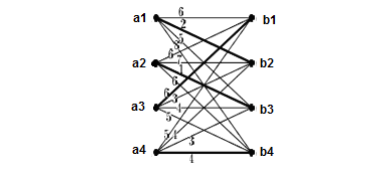
\includegraphics{graph.png} (graph from \cite{image} mentioned before)


% dummy text

% The bibiliography
\begin{thebibliography}{2}
\bibitem{Alpin} 
\textcolor{red}{Alpin, J., and Mubarakzianow, R. "The bases of weighted graphs." Discrete Mathematics, vol. 175, no. 1–3, 1997, pp. 1-11, https://doi.org/10.1016/S0012-365X(96)00282-8.}
\bibitem{image}
Rahimi, Z., and Taghipour, K., and Khadivi, S., and Afhami, N. "Document and sentence alignment in comparable corpora using bipartite graph matching." 6th International Symposium on Telecommunications, 2012, pp. 817-821, 10.1109/ISTEL.2012.6483098. 
\bibitem{latexcompanion} 
Gale, D., and L. S. Shapley. “College Admissions and the Stability of Marriage.” The American Mathematical Monthly, vol. 69, no. 1, Mathematical Association of America, 1962, pp. 9–15, https://doi.org/10.2307/2312726
\bibitem{3} 
\textcolor{red}{Mingwen, W. "A new algorithm for stable assignment." International Journal of Computer Mathematics, vol. 66, no.1-2, 1998, pp. 1-7, DOI: 10.1080/00207169808804620}
\end{thebibliography}

\end{document}
